\documentclass{standalone}

\usepackage{amsmath, amssymb, amsfonts, amscd, amsthm, bigints, units}
%!TEX encoding = UTF-8 Unicode
\usepackage{tikz}
\usepackage{tikz-cd}
\usepackage{tikz3dcs-pp}
\usepackage{pgfplots}
\usepackage{xcolor, eecolors}
\usepackage{math, lrmath}

\usepackage{pgfplots}
\usepgfplotslibrary{patchplots}
\pgfplotsset{compat=1.15}

\usetikzlibrary{calc, intersections}

\usetikzlibrary{decorations.pathmorphing,calc,shapes,positioning,fit,arrows,fadings,decorations.pathreplacing,decorations.pathmorphing,intersections,patterns, trees}
\usetikzlibrary{decorations.markings}

\usepackage{marvosym}

%%%%%%%%My Tikz definitions%%%%%%%%%%%%%%%%%
\tikzset{->-/.style={decoration={
  markings,
  mark=at position #1 with {\arrow{latex}}},postaction={decorate}}}
  %
\tikzset{
    %Define standard arrow tip
    >=stealth',
    %Define style for boxes
    punkt/.style={
           rectangle,
           rounded corners,
           draw=black, very thick,
           text width=7.5em,
           minimum height=2em,
           text centered},
    % Define arrow style
    pil/.style={
           ->,
           thick,
           shorten <=2pt,
           shorten >=2pt,}
}
%%%
%%3d drawings %%%
\newcommand\pgfmathsinandcos[3]{%
  \pgfmathsetmacro#1{sin(#3)}%
  \pgfmathsetmacro#2{cos(#3)}%
}
\newcommand\LongitudePlane[3][current plane]{%
  \pgfmathsinandcos\sinEl\cosEl{#2} % elevation
  \pgfmathsinandcos\sint\cost{#3} % azimuth
  \tikzset{#1/.style={cm={\cost,\sint*\sinEl,0,\cosEl,(0,0)}}}
}
\newcommand\LatitudePlane[3][current plane]{%
  \pgfmathsinandcos\sinEl\cosEl{#2} % elevation
  \pgfmathsinandcos\sint\cost{#3} % latitude
  \pgfmathsetmacro\yshift{\cosEl*\sint}
  \tikzset{#1/.style={cm={\cost,0,0,\cost*\sinEl,(0,\yshift)}}} %
}
\newcommand\DrawLongitudeCircle[2][1]{
  \LongitudePlane{\angEl}{#2}
  \tikzset{current plane/.prefix style={scale=#1}}
   % angle of "visibility"
  \pgfmathsetmacro\angVis{atan(sin(#2)*cos(\angEl)/sin(\angEl))} %
  \draw[current plane] (\angVis:1) arc (\angVis:\angVis+180:1);
  \draw[current plane,dashed] (\angVis-180:1) arc (\angVis-180:\angVis:1);
}
\newcommand\DrawLatitudeCircle[2][1]{
  \LatitudePlane{\angEl}{#2}
  \tikzset{current plane/.prefix style={scale=#1}}
  \pgfmathsetmacro\sinVis{sin(#2)/cos(#2)*sin(\angEl)/cos(\angEl)}
  % angle of "visibility"
  \pgfmathsetmacro\angVis{asin(min(1,max(\sinVis,-1)))}
  \draw[current plane] (\angVis:1) arc (\angVis:-\angVis-180:1);
  \draw[current plane,dashed] (180-\angVis:1) arc (180-\angVis:\angVis:1);
}
%%%%


\begin{document}
%	\begin{tikzpicture}
%       		%
%		\def\N{7}
%       		\def\thetaDW4{60}
%       		\def\dDW4{5}
%       		\def\thetaAdS4{90}
%       		\def\dAdS4{5}
%       		%
%		\node[label=below:$\mathrm{AdS}_2 \times \Sigma_\mathfrak{g}$, fill, draw, circle, minimum size=0.01, inner sep=1] (AdS2) at (0,0) {};
%       		\node[fill, draw, circle, minimum size=0.01, inner sep=1] (DW4) at ($(AdS2) + (\thetaDW4:\dDW4)$) {};
%       		\node[label=above:$\mathrm{AdS}_4$, fill, draw, circle, minimum size=0.01, inner sep=1] (AdS4) at ($(AdS2) + (\thetaAdS4:\dAdS4)$) {};
%		\node at (1.2,5.15) {$\textcolor{blue}{m^2 \varphi^2}$};
%		\node at (-.55, 3.5) {$\textcolor{red}{\bigintss\!\! F = q}$};
%
%	       \def\outDW4{-75}
%	       \def\outAdS4{-85}
%	       \def\inAdS2{75}
%		%
%		       \draw[->-=.45, color= red] (DW4) to [out=\outDW4, in=\inAdS2] (AdS2);
%		       \draw[->-=.45, color= red] (AdS4) to [out=\outAdS4, in=\inAdS2] (AdS2);
%		       \draw[->-=.55] (AdS4) to [out=0, in=\inAdS2] (AdS2);
%
%	       \path[name path=AdS4DW4, draw, color = blue, ->-=.4] (AdS4) to[out=10, in=190] (DW4);
%	       
%	       \draw[->-=.6] plot [smooth, tension=.3] coordinates { (AdS4) (.3, 4.9) (0.9, 4.7) (1.5,4.3) ($(DW4)-(.2,.8)$) ($(AdS2)+(.3,.7)$) (AdS2)};
%		%
%%       		\foreach \i in {1,...,\N}{
%%           					\path[name path=ray\i] (AdS2) -- ++({\thetaDW4+\i*(\thetaAdS4-\thetaDW4)/(\N + 1)}:\dAdS4+1);
%%           					\path [name intersections={of=AdS4DW4 and ray\i,by=int\i}];
%%           					\pgfmathparse{\outDW4+\i*(\outAdS4-\outDW4)/(\N + 1)}
%%           					\draw[->-=.45] (int\i) to[out=\pgfmathresult, in=\inAdS2] (AdS2);
%%       		}
%		%
%   	\end{tikzpicture}
   
   %%%%%
	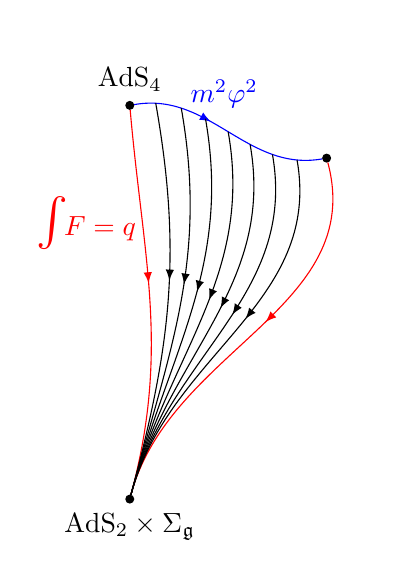
\begin{tikzpicture}
       		%
		\def\N{7}
       		\def\thetaDW4{60}
       		\def\dDW4{5}
       		\def\thetaAdS4{90}
       		\def\dAdS4{5}
       		%
		\node[label=below:$\mathrm{AdS}_2 \times \Sigma_\mathfrak{g}$, fill, draw, circle, minimum size=0.01, inner sep=1] (AdS2) at (0,0) {};
       		\node[fill, draw, circle, minimum size=0.01, inner sep=1] (DW4) at ($(AdS2) + (\thetaDW4:\dDW4)$) {};
       		\node[label=above:$\mathrm{AdS}_4$, fill, draw, circle, minimum size=0.01, inner sep=1] (AdS4) at ($(AdS2) + (\thetaAdS4:\dAdS4)$) {};
		\node at (1.2,5.15) {$\textcolor{blue}{m^2 \varphi^2}$};
		\node at (-.55, 3.5) {$\textcolor{red}{\bigintss\!\! F = q}$};

	       \def\outDW4{-75}
	       \def\outAdS4{-85}
	       \def\inAdS2{75}
		%
		       \draw[->-=.45, color= red] (DW4) to [out=\outDW4, in=\inAdS2] (AdS2);
		       \draw[->-=.45, color= red] (AdS4) to [out=\outAdS4, in=\inAdS2] (AdS2);

	       \path[name path=AdS4DW4, draw, color = blue, ->-=.4] (AdS4) to[out=10, in=190] (DW4);
		%
       		\foreach \i in {1,...,\N}{
           					\path[name path=ray\i] (AdS2) -- ++({\thetaDW4+\i*(\thetaAdS4-\thetaDW4)/(\N + 1)}:\dAdS4+1);
           					\path [name intersections={of=AdS4DW4 and ray\i,by=int\i}];
           					\pgfmathparse{\outDW4+\i*(\outAdS4-\outDW4)/(\N + 1)}
           					\draw[->-=.45] (int\i) to[out=\pgfmathresult, in=\inAdS2] (AdS2);
       		}
		%
   	\end{tikzpicture}

   
   %%%%%
   
%	\begin{tikzpicture}
%  			\node[label=below:$x_1$]  (x1) at (6,0)  {$\bullet$};
%  			\node[label=above:$x_0$]  (x0) at (9,4)  {$\bullet$};  
%  			\draw (x1.center) to [out=5,in=-90]++(2.8,1.8) to[out=90,in=-95](x0.center);
%  			\draw (x1.center) to [out=10,in=-110]++(2.6,2) to[out=70,in=-103](x0.center); 
%  			\draw (x1.center) to [out=15,in=-105](x0.center);
%  			\draw (x1.center) to [out=30,in=-150](x0.center);
%  			\draw (x1.center) to [out=45,in=-170](x0.center); 
%  			\draw (x1.center) to [out=50,in=-105]++(1.2,3)to [out=75,in=-172](x0.center); 
%  			\draw (x1.center) to [out=55,in=-100]++(1.0,3) to[out=80,in=-175](x0.center); 
%  			\draw (x1.center) to [out=60,in=-90]++(0.8,3) to[out=90,in=-180] (x0.center); 
%	\end{tikzpicture}

\end{document}